\section{Charge balance and efficiency}\label{sec:efficiency}
\sectionstate{partial}{PLAN\_38 (\texttt{38\_xy\_charge\_balance.py}); efficiency maps (\texttt{08}, \texttt{09}); edge study \texttt{32\_edge\_fringe\_field.py} (hits angle, D4)}
\intent{How the charge divides between the two views, and where each chamber is efficient. Hits are the right input
here (detection, amplitude); positions come from the M3 reference, not from the chamber.}

\subsection{X/Y charge balance}
\tbw{$f=q_X/(q_X+q_Y)$: median 0.487 (det3) and 0.531 (det2), $\sigma_{68}=0.07$, flat in position and angle; three charge proxies agree.}
\begin{figure}[t]
  \centering
  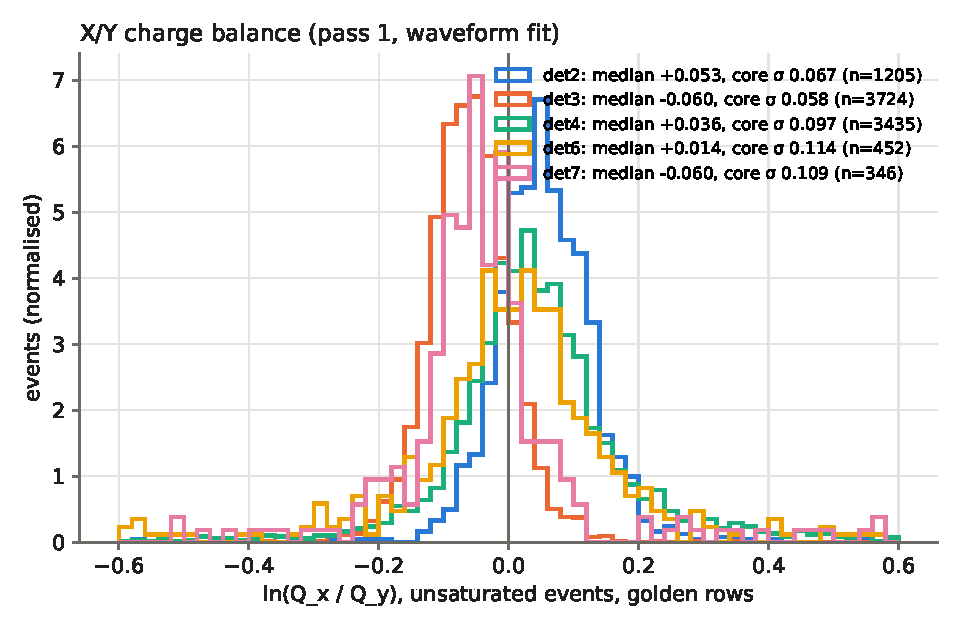
\includegraphics[width=0.6\linewidth]{charge_balance}
  \caption{\tbw{X/Y charge balance.}}
  \label{fig:balance}
\end{figure}

\subsection{Efficiency and maps}
\tbw{Detection efficiency per chamber; maps; the edge turn-on. Efficiency within 5\,mm:
\requote{93/92/42/75/57\,\%} (det3/2/4/6/7). det4's low value is its non-amplifying area (\cref{sec:det4}).}
\analysis{D1}{re-quote from the reproduced r06 products}
\analysis{D4}{edge angle tilt with wft angles}
\begin{figure}[t]
  \centering
  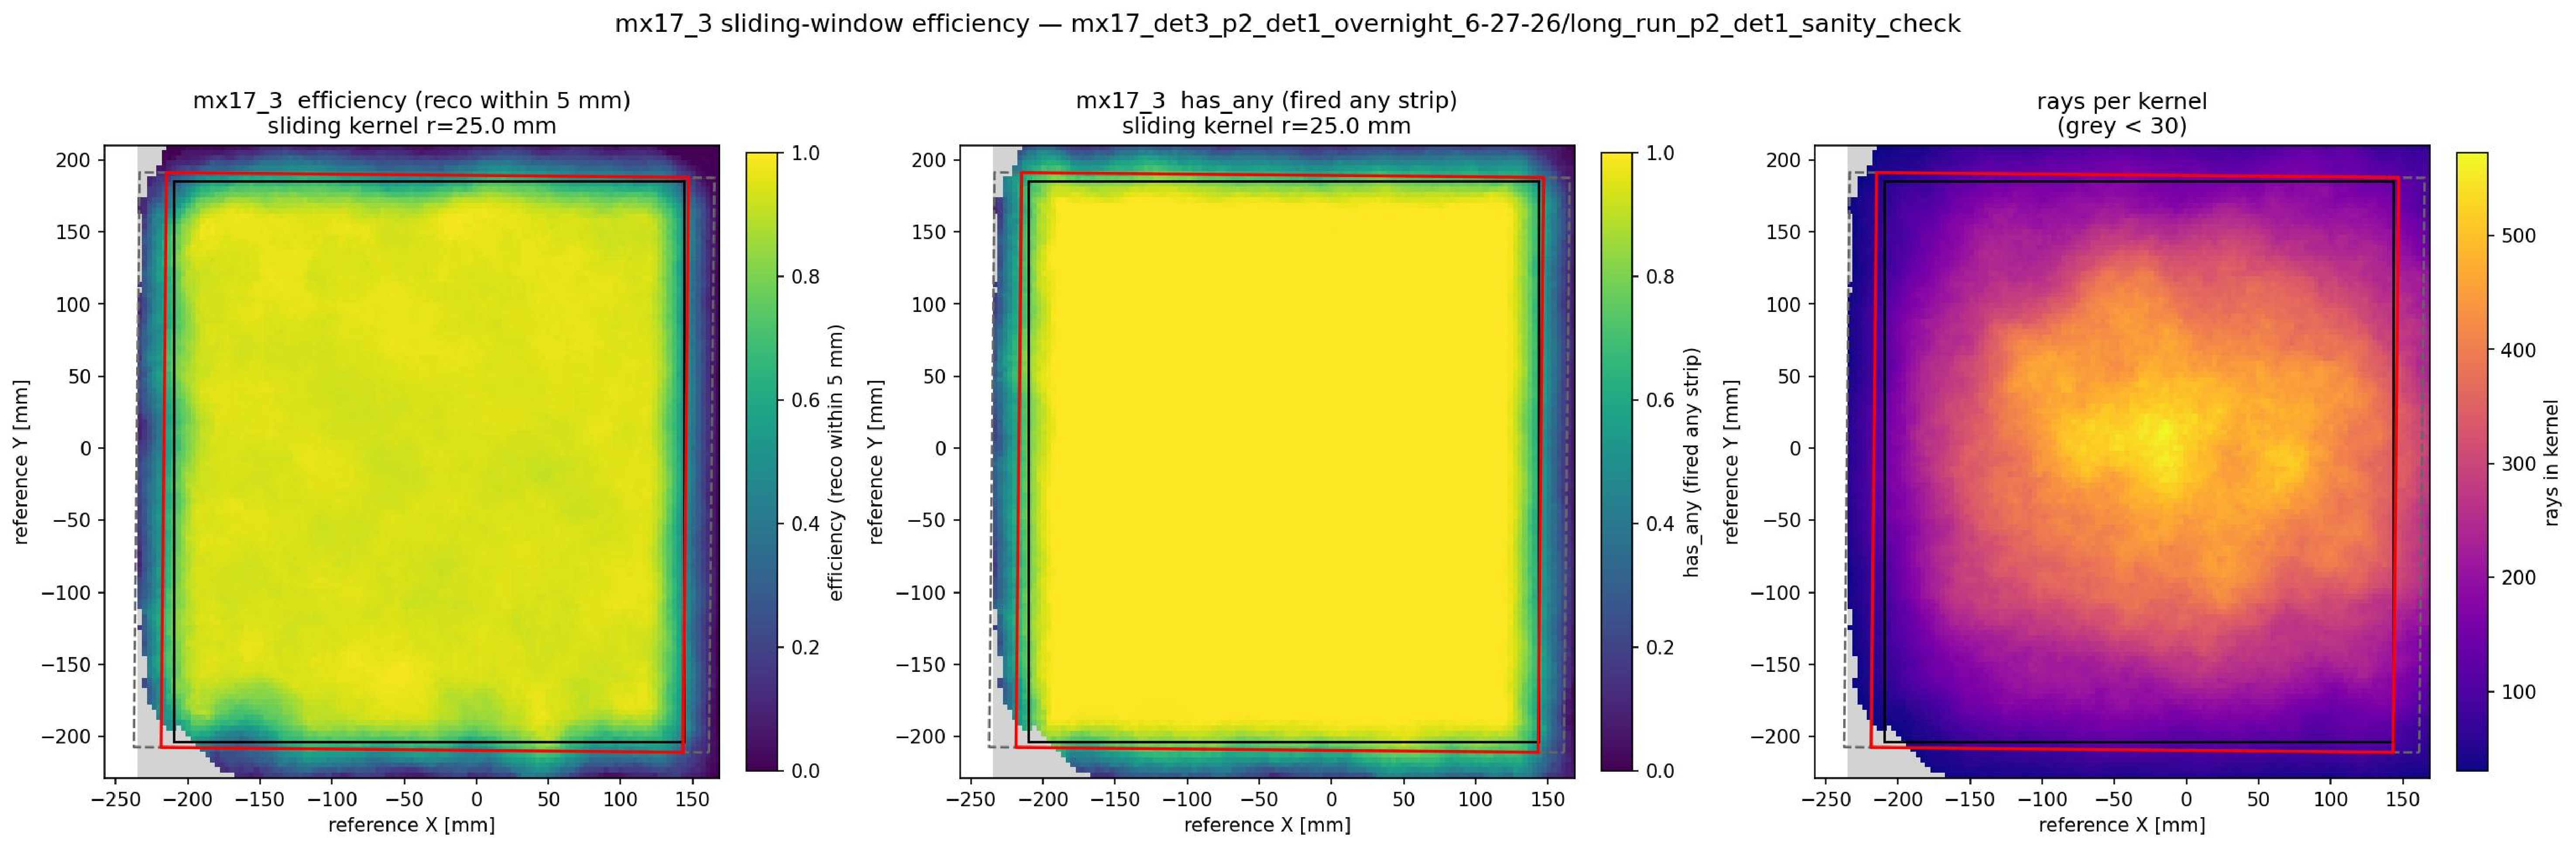
\includegraphics[width=0.7\linewidth]{efficiency_map}
  \caption{\tbw{Efficiency map (det3).}}
  \label{fig:effmap}
\end{figure}
\begin{figure}[t]
  \centering
  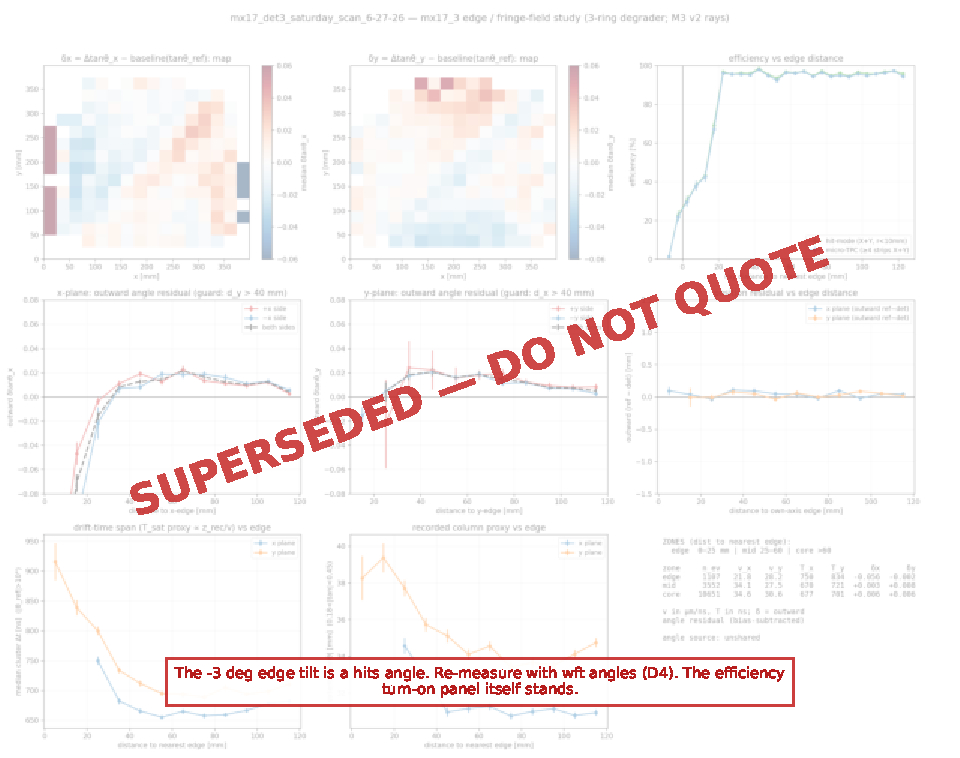
\includegraphics[width=0.7\linewidth]{edge_turnon}
  \caption{\tbw{Efficiency turn-on at the chamber edge.}}
  \label{fig:edge}
\end{figure}
